\subsection{Sistema operativo de tiempo real}

Un sistema operativo en tiempo real (RTOS por sus siglas en inglés) es un tipo de sistema operativo diseñado para gestionar tareas de manera determinista, garantizando que ciertas operaciones se completen dentro de plazos definidos \cite{rtos}. A diferencia de los sistemas operativos convencionales, donde la prioridad de las tareas puede variar según la carga del sistema, un RTOS garantiza que las tareas críticas se ejecuten en tiempo y forma según su prioridad. \\

Los RTOS son fundamentales en aplicaciones embebidas donde es crucial que las respuestas a eventos externos, como la activación de un sensor o una interrupción, se produzcan dentro de tiempos predeterminados. Estos sistemas son ampliamente utilizados en sectores como el automotriz, la aviación, las telecomunicaciones, y los sistemas médicos. \\

Algunas características clave de los RTOS incluyen:

\begin{itemize}
    \item \textbf{Determinismo}: El comportamiento predecible en cuanto a la ejecución de tareas es esencial. Un RTOS asegura que las tareas se ejecuten de acuerdo con una planificación estricta, cumpliendo con los plazos impuestos por el sistema.

    \item \textbf{Multitarea}: Un RTOS es capaz de manejar múltiples tareas concurrentemente, priorizando aquellas que son más críticas para el sistema.

    \item \textbf{Gestión de interrupciones}: La rápida respuesta a interrupciones de hardware es vital en un RTOS. Estos sistemas permiten que las tareas de mayor prioridad respondan rápidamente a eventos externos, sin demoras significativas.

    \item \textbf{Uso eficiente de recursos}: Dado que los RTOS suelen implementarse en sistemas embebidos con recursos limitados, están optimizados para ser ligeros y eficientes en términos de memoria y procesamiento.

\end{itemize}


En la figura \ref{fig:freertos_tasks} se muestra un ejemplo de un RTOS realizando asignación de tareas con distintas prioridades e interactuando con una interrupción por hardware. 

\begin{figure}[H]
    \centering
    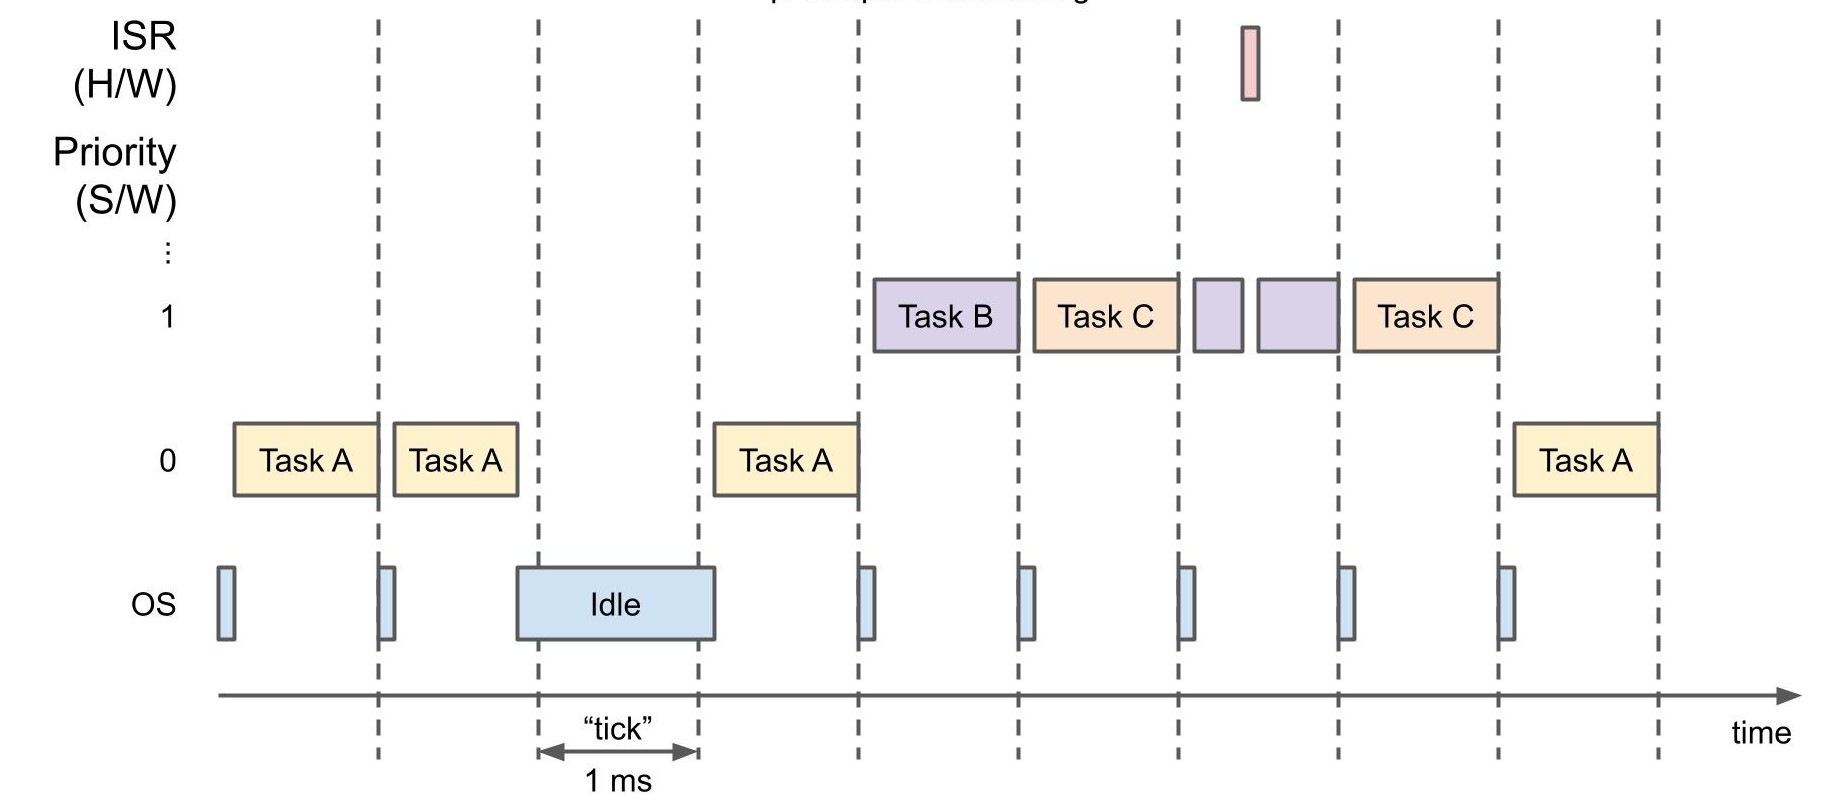
\includegraphics[width = \linewidth]{img/freertos_tasks.jpeg}
    \caption{Asignación de tareas por prioridades en un RTOS}
    \label{fig:freertos_tasks}
\end{figure}


